\documentclass[submit]{harvardml}

\course{CS181-S21}
\assignment{Assignment \#4}
\duedate{7:59pm EST, March 19, 2021} 

\usepackage[OT1]{fontenc}
\usepackage[colorlinks,citecolor=blue,urlcolor=blue]{hyperref}
\usepackage[pdftex]{graphicx}
\usepackage{graphicx}
\usepackage{caption}
\usepackage{fullpage}
\usepackage{soul}
\usepackage{amsmath}
\usepackage{amssymb}
\usepackage{color}
\usepackage{todonotes}
\usepackage{listings}
\usepackage{common}
\usepackage{float}

\usepackage[mmddyyyy,hhmmss]{datetime}

\definecolor{verbgray}{gray}{0.9}

\lstnewenvironment{csv}{
  \lstset{backgroundcolor=\color{verbgray},
  frame=single,
  framerule=0pt,
  basicstyle=\ttfamily,
  columns=fullflexible}}{}
 
\begin{document}

\begin{center}
{\Large Homework 4: SVM, Clustering, and Ethics}\\
\end{center}

\subsection*{Introduction}

This homework assignment will have you work with SVMs, 
clustering, and engage with the ethics lecture.  We encourage you to
read Chapters 5 and 6 of the course textbook.

Please submit the \textbf{writeup PDF to the Gradescope assignment `HW4'}. Remember to assign pages for each question.

Please submit your \textbf{\LaTeX\ file and code files to the Gradescope assignment `HW4 - Supplemental'}. 

\newpage

%%%%%%%%%%%%%%%%%%%%%%%%%%%%%%%%%%%%%%%%%%%%%
% Problem 1
%%%%%%%%%%%%%%%%%%%%%%%%%%%%%%%%%%%%%%%%%%%%%
\begin{problem}[Fitting an SVM by hand, 10pts]

  For this problem you will solve an SVM by hand, relying on principled rules and SVM properties. 
  For making plots, however, you are allowed to use a computer or other graphical tools.

Consider a dataset with the following 7 data points each with $x \in \reals$ and $y \in \{ -1, +1 \}$ : \[\{(x_i, y_i)\}_{i = 1}^7 =\{(-3 , +1) , (-2 , +1 ) , (-1,  -1 ), (0, +1), ( 1 , -1 ), ( 2 , +1 ) , (3 , +1 )\}\] Consider
mapping these points to $2$ dimensions using the feature vector $\bphi(x) =  (x, -\frac{8}{3}x^2 + \frac{2}{3}x^4 )$. The hard margin classifier training problem is:
%
\begin{align*}
  &\min_{\mathbf{w}, w_0} \frac{1}{2}\|\mathbf{w}\|_2^2 \label{eq:dcp} \\
  \quad \text{s.t.} \quad & y_i(\mathbf{w}^\top \bphi(x_i) + w_0) \geq 1,~\forall i \in \{1,\ldots, n\}\notag
\end{align*}

Make sure to follow the logical structure of
the questions below when composing your answers, and to justify each step.

\begin{enumerate}
\item Plot the transformed training data in $\reals^2$ and draw the
  optimal decision boundary of the max margin classifier. You can
  determine this by inspection (i.e. by hand, without actually doing
  any calculations).

\item What is the value of the margin achieved by the optimal decision
  boundary found in Part 1?

\item Identify a unit vector that is orthogonal to the decision boundary.

\item Considering the discriminant
  $h(\bphi(x);\boldw,w_0)=\boldw^\top\bphi(x) +w_0$, give an
  expression for {\em all possible} $(\boldw,w_0)$ that define the
  optimal decision boundary from 1.1.  Justify your answer.

  Hint: The boundary is where the discriminant is equal to 0.  Use
  what you know from 1.1 and 1.3 to solve for $\boldw$ in terms of
  $w_0$.  (If you solve this problem in this way, then $w_0$
  corresponds to your free parameter to describe the set of all
  possible $(\boldw,w_0)$.)
  
\item Consider now the training problem for this dataset. Using your
  answers so far, what particular solution to $\boldw$ will be optimal
  for the optimization problem?

\item What is the corresponding optimal value of $w_0$ for the
  $\boldw$ found in Part 5 (use your result from Part 4 as guidance)?
  Substitute in these optimal values and write out the discriminant
  function $h(\bphi(x);\boldw,w_0)$ in terms of the variable $x$ .


\item Which points could possibly be support vectors of the classifier?  Confirm that
  your solution in Part 6 makes the constraints above tight---that is,
  met with equality---for these candidate points.

\end{enumerate}

\end{problem}


\newpage

\subsection*{Solution 1}
\begin{enumerate}
    \item \textbf{Plot the transformed training data in R2 and draw the optimal decision boundary of the max margin classifier}\\
    
    The data was plotted on a 2d plane, with a decision boundary drawn at $\Phi (x) = 1$, the classes are colored with blue representing the $ Y = 1$ class and red representing the $Y = -1$ class.
    \begin{figure}[H]
        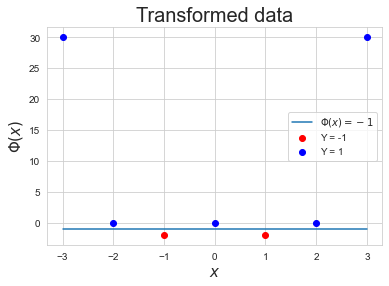
\includegraphics[width=10cm]{hw4/img/hw4p1.png}
        \centering
    \end{figure}
    
    \item \textbf{What is the value of the margin achieved by the optimal decision boundary found in Part 1?}\\
    
    The value of the margin found in part 1 is $1$.\\
    
    \item \textbf{Identify a unit vector that is orthogonal to the decision boundary.}\\
    
    The unit vector $\vec{V} = [0,1]$ is orthogonal to the decision boundary.\\
    
    \item \textbf{Give an expression for \textit{all possible} (w, w0) that define the optimal decision boundary from 1.1}\\
    
    First, we know that at the boundary, $W\Phi(x) + w_0 = 0$, we also know that our $W$ and the vector $\vec{V} = [0,1]$ are orthogonal to the decision boundary. Therefore, we know $W \propto V$, as we can set $W = [w_a, w_b]$ we can use $\vec{V}$ to say that $W = [0, w_b]$.
    
    Let's look at the case where we are at the boundary, here $\Phi(x)_2 = -1$. By using our value of $W$ from before we can now write: $w_b(-1) + w_0 = 0$ for a point at the decision boundary.
    
    \begin{align*}
        w_b &= w_0 \\
        W &= [0, w_0]
    \end{align*}
    
    This defines the set of all $W$ and $w_0$ for the optimal decision boundary
    
    \item \textbf{Using your answers so far, what particular solution to $W$ will be optimal for the optimization problem?}\\
    
    Using the equation above:
    
    \begin{align*}
        \min_{\mathbf{w}, w_0} \frac{1}{2}\|\mathbf{w}\|_2^2 \quad \text{s.t.} \quad & y_i(\mathbf{w}^\top \bphi(x_i) + w_0) \geq 1,~\forall i \in \{1,\ldots, n\}
    \end{align*}
    
    We can simplify the optimisation to only work over the $w_0$ from part 4, $\bphi(x_{i})_2$ represents the $i^{th}$ element of x in the second row (i.e. only those transformed by the basis function). 
    \begin{align*}
        &\min_{\mathbf{w_0}} \mathbf{w_0} \quad \text{s.t.} \quad & y_i(w_0 \bphi(x_{i})_2 + w_0) \geq 1,~\forall i \in \{1,\ldots, n\} \\
        &= \min_{\mathbf{w_0}} \mathbf{w_0} \quad \text{s.t.} \quad & y_i w_0 ( \bphi(x_{i})_2 + 1) \geq 1,~\forall i \in \{1,\ldots, n\} \\
    \end{align*}
    
    Using the points from the graph above, we can see that the minimum $w_0$ that satisfies is at 1, $\therefore \quad w = [0,1]$. 
    
    \item \textbf{What is the corresponding optimal value of $w_0$ for the $w$ found in part 5?}\\
    
    The optimal $w$ found in part 5 was $ w = [0,1]$, we can substitute this into the discriminant function to get:\\
    
    \begin{align*}
        h(\bphi(x);\boldw,w_0) &= \boldw^\top\bphi(x) +w_0\\
        h(\bphi(x);\boldw,w_0) &= 1\bphi(x)_2 + 1 \\
        h(\bphi(x);\boldw,w_0) &= \frac{-3}{8}x^2 + \frac{2}{3} x^4 + 1 \\
    \end{align*}
    
    \item \textbf{Which points could possibly be support vectors of the classifier?  Confirm that your solution in Part 6 makes the constraints above tight—that is, met with equality—for these candidate points.}\\
     
    There are 5 points that could make suitable support vectors: $\{ (-2 , +1 ) , (-1,  -1 ), (0, +1), ( 1 , -1 ), ( 2 , +1 )\}$, these 5 points surround the decision boundary. We can justify that they are valid support vectors by plugging in their x,y vales into $y(\frac{-3}{8}x^2 + \frac{2}{3} x^4 + 1)$ and show that it is $\geq 1$.
    \begin{align*}
        1(\frac{-3}{8}(-2)^2 + \frac{2}{3} (-2)^4 + 1) &= 1 \\
        -1(\frac{-3}{8}(-1)^2 + \frac{2}{3} (-1)^4 + 1) &= 1 \\
        1(\frac{-3}{8}(0)^2 + \frac{2}{3} (0)^4 + 1) &= 1 \\
        -1(\frac{-3}{8}(1)^2 + \frac{2}{3} (1)^4 + 1) &= 1 \\
        1(\frac{-3}{8}(2)^2 + \frac{2}{3} (2)^4 + 1) &= 1 \\
    \end{align*}
\end{enumerate}

%%%%%%%%%%%%%%%%%%%%%%%%%%%%%%%%%%%%%%%%%%%%%
% Problem 2
%%%%%%%%%%%%%%%%%%%%%%%%%%%%%%%%%%%%%%%%%%%%%

\begin{problem}[K-Means and HAC, 20pts]


For this problem you will implement K-Means and HAC from scratch to cluster image data. You may use \texttt{numpy} but no third-party ML implementations (eg. \texttt{scikit-learn}).

We've provided you with a subset of the MNIST dataset, a collection of
handwritten digits used as a benchmark for image recognition (learn more at
\url{http://yann.lecun.com/exdb/mnist/}). MNIST is widely used in supervised learning, and modern algorithms do very well. 

You have been given
representations of MNIST images, each of which is a $784\times1$
greyscale handwritten digit from 0-9. Your job is to implement K-means and HAC on MNIST, and to test whether these relatively
simple algorithms can cluster similar-looking images together.

The code in \texttt{T4\_P2.py} loads the images into your environment into two arrays -- \texttt{large\_dataset}, a 5000x784 array, will be used for K-means, while \texttt{small\_dataset}, a 300x784 array, will be used for HAC. In your code, you should use the $\ell_2$ norm (i.e. Euclidean distance) as your distance metric.

\textbf{Important:} Remember to include all of your plots in your PDF submission!

\textbf{Checking your algorithms:} Instead of an Autograder file, we have provided a similar dataset, \texttt{P2\_Autograder\_Data}, and some visualizations, \texttt{HAC\_visual} and \texttt{KMeans\_visual}, for how K-means and HAC perform on this data. Run your K-means (with $K=10$ and \texttt{np.random.seed(2)}) and HAC on this second dataset to confirm your answers against the provided visualizations. Do \textbf{not} submit the outputs generated from \texttt{P2\_Autograder\_Data}. Load this data with \texttt{data = np.load(`P2\_Autograder\_Data.npy')}.

\begin{enumerate}

\item Starting at a random initialization and $K = 10$, plot
  the K-means objective function (the residual sum of squares) as a function of iterations and verify
  that it never increases.

\item Run K-means for 5 different restarts for different values of $K = 5, 10, 20$. Make a plot of the final K-means objective value after your algorithm converges (y-axis) v. the values of K (x-axis), with each data point having an error bar. To compute these error bars, you will use the $5$ final objective values from the restarts for each $K$ to calculate a standard deviation for each $K$.

  How does the final value of the objective function and its standard deviation change with $K$? (Note: Our code takes ~10 minutes to run for this part.)
  
\item For $K=10$ and for 3 random restarts, show the mean
  image (aka the centroid) for each cluster.
  To render an image, use the pyplot
  \texttt{imshow} function. There should be 30 total images. Include all of these images
  as part of a single plot; your plot must fit on one page.

\item Repeat Part 3, but before running K-means, standardize or center the data such that each pixel has mean
  0 and variance 1 (for any pixels with zero variance, simply divide by 1). For $K=10$ and 3 random restarts,
  show the mean image (centroid) for each cluster. Again, present the 30 total images in a single plot. Compare to Part 3: How do the centroids visually differ? Why? 

\item Implement HAC for min, max, and centroid-based linkages. Fit these models to the \texttt{small\_dataset}. 
  For each of these 3 linkage criteria, find the mean image for each cluster when using $10$ clusters. Display these images (30 total) on a single plot.
  How do these centroids compare to those found with K-means? \textbf{Important Note:} For this part ONLY, you may use \texttt{scipy}'s \texttt{cdist} function to calculate Euclidean distances between every pair of points in two arrays.

\item For each of the 3 HAC linkages (max/min/centroid), plot
  "Distance between most recently merged clusters" (y-axis) v. "Total number of merges completed" (x-axis).
  Does this plot suggest that there are any  natural cut points? 

\item For each of the max and min HAC linkages, make a plot of "Number of images in cluster" (y-axis) v. "Cluster index" (x-axis) reflecting the assignments during
	the phase of the algorithm when there were $K=10$
	clusters. Intuitively, what do these plots tell you about the difference between the clusters produced by the max and min linkage criteria?

\item For your K-means with $K = 10$ model and HAC min/max/centroid models using $10$ clusters on the \texttt{small\_dataset} images, use the \texttt{seaborn} module's \texttt{heatmap} function to plot a confusion matrix of clusters v. actual digits. This is 4 matrices, one per method, each method vs. true labeling. The cell at the $i$th row, $j$th column of your confusion matrix is the number of times that an image with the true label of $j$ appears in cluster $i$. How well do the different approaches match the digits? Is this matching a reasonable evaluation metric for the clustering?  Explain why or why not.   
  
\end{enumerate}

\end{problem}

\subsection*{Solution 2}

\begin{enumerate}
    \item \textbf{Plot the K-Means objective function as function of iterations and verify that it never increases.}\\
    
    Starting at a random initialisation, we can see the loss decreasing steadily with epoch, the graph is monotonic and the loss never increases at any point.
    \begin{figure}[H]
        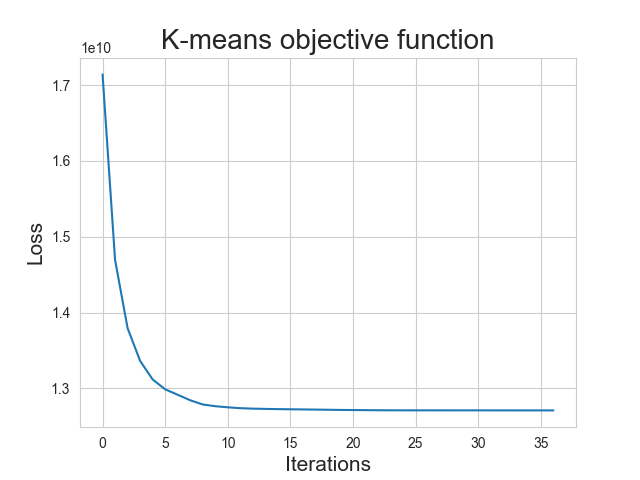
\includegraphics[width=8cm]{hw4/img/p2_1.png}
        \centering
    \end{figure}
    
    \item \textbf{Run  K-means  for  5  different  restarts  for  different  values  of K=  5,10,20.   Make  a  plot  of  the final K-means objective value after your algorithm converges (y-axis) v.  the values of K (x-axis),with each data point having an error bar.}
    
    The standard deviation of each K is plotted as vertical error bars, the plot of the loss at each K is represented by an X mark.
    \begin{figure}[H]
        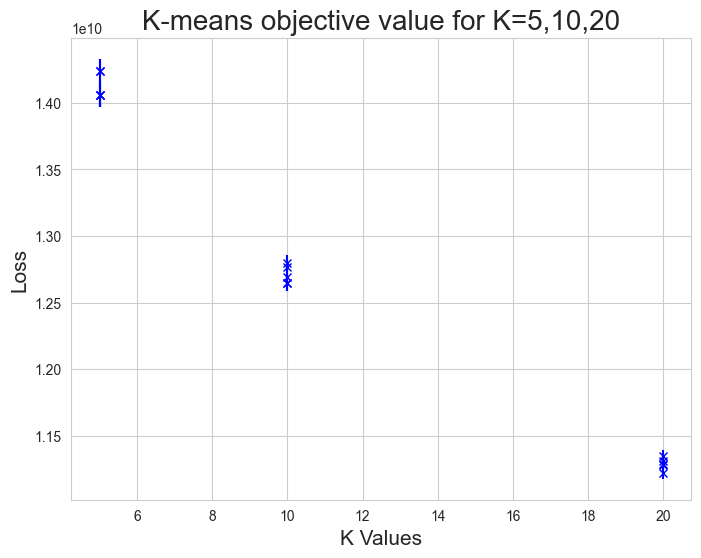
\includegraphics[width=8cm]{hw4/img/p2_2.png}
        \centering
    \end{figure}
    
    \newpage
    \item \textbf{ ForK= 10 and for 3 random restarts, show the mean image (aka the centroid) for each cluster.}
    
    Each column represents a new restart, initialised using random values. Each row represents the mean value of a cluster. You can see each of the mean values roughly equaling a different underlying true value (i.e. they are somewhat displaying each of the 10 digits).
    
    \begin{figure}[H]
        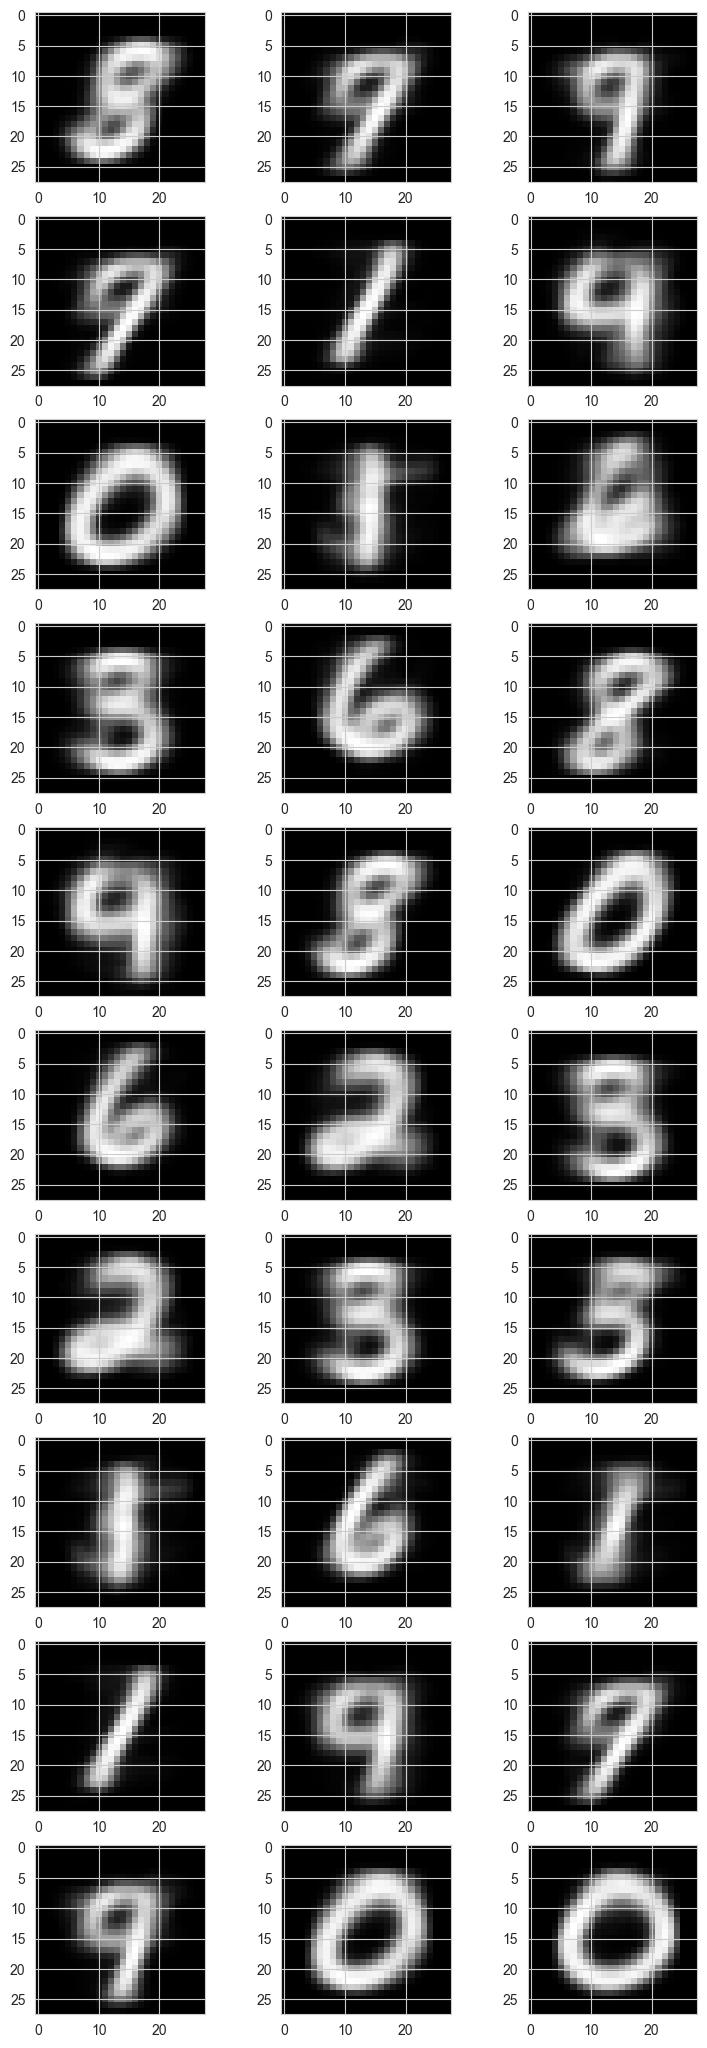
\includegraphics[height=20cm]{hw4/img/p2_3.png}
        \centering
    \end{figure}
    
    \newpage
    \item \textbf{Repeat Part 3, but before running K-means, standardize or center the data such that each pixel has mean 0 and variance 1.}
    
    As all the images are standardised, only the bits of a datapoint that are different to the majority of other images remain. The centroids now are picking up the most common outlier pixels.
    
    \begin{figure}[H]
        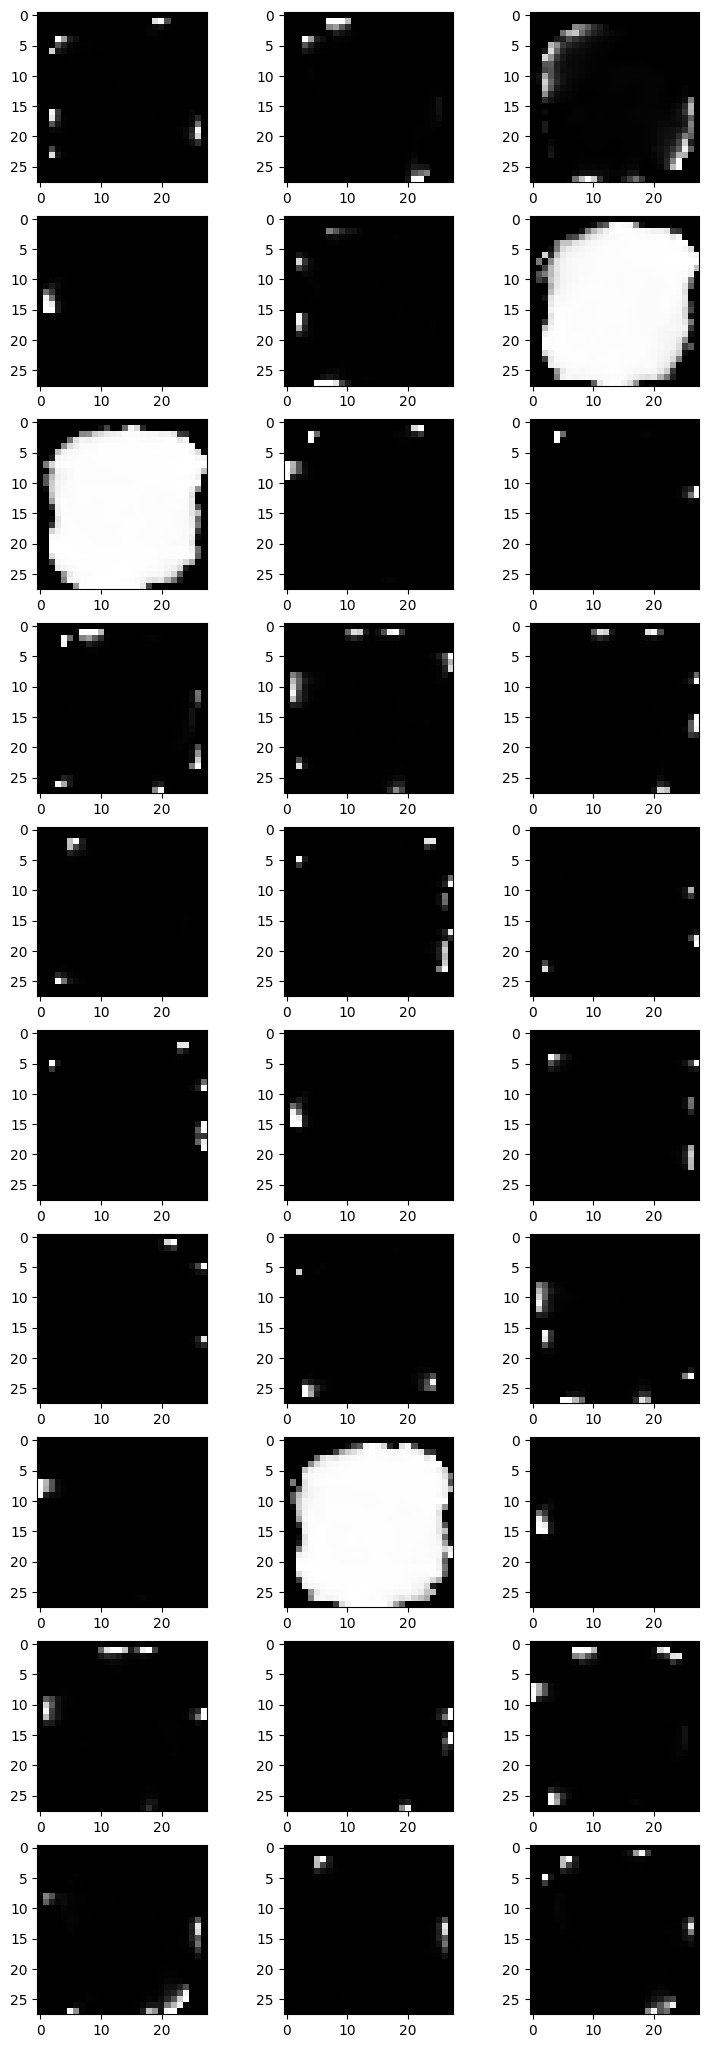
\includegraphics[height=20cm]{hw4/img/p2_4.png}
        \centering
    \end{figure}
    
    
    
\end{enumerate}
%%%%%%%%%%%%%%%%%%%%%%%%%%%%%%%%%%%%%%%%%%%%%
% Problem 3
%%%%%%%%%%%%%%%%%%%%%%%%%%%%%%%%%%%%%%%%%%%%%

\begin{problem}[Ethics Assignment, 15pts]

Read the article ``\href{https://www.bloomberg.com/graphics/2016-amazon-same-day/}{Amazon Doesn’t Consider the Race of Its Customers. Should It?}''. Please write no more than 1 concise paragraph each in response to the below reflection questions.  We do not expect you to do any outside research, though we encourage you to connect to lecture materials and the reading for the module where relevant.

\begin{enumerate}
    \item Some people think that Amazon’s process for determining which neighborhoods would receive same-day delivery was wrongfully discriminatory, but others disagree.  Based on our definitions and discussions from lecture, do you believe that Amazon's same-day delivery process was wrongfully discriminatory? Explain your reasoning.
    
    % NJ:  Lyndal wrote the above.  I clarified to make it clear that students should connect to definitions from class. 
    
    \item Basing decisions about how to treat others on social group membership often strikes us as being wrongfully discriminatory. For example, most people would say that refusing to hire someone because they are a woman is wrongful discrimination, at least under normal circumstances.
    
    However, there are some cases in which some people argue that social group membership \emph{should} be taken into consideration when deciding how to treat others.  The title of the article poses the question: Do you think that should Amazon consider the race of its customers in its same-day delivery processes? If so, then how? 
    
    % NJ:  I edited this a lot to be more explicit that we want students to think more along the lines of equity.  The question as it was originally phrased confused me because it made me feel like I needed to choose some kind of policy that harmed marginalized groups (I didn't like the line "even if it ends up disadvantaging members of one group"... because it implies that equity is necessarily "damaging" or taking away.)
    
    % Lyndal's original question: Basing decisions about how to treat others on social group membership often strikes us as wrongfully discriminatory. For example, most people would say that refusing to hire someone because they are a woman is wrongful discrimination, at least under normal circumstances. However, there are cases in which deciding how to treat people on the basis of social group membership does not strike most people as unfair, even if it ends up disadvantaging members of one group relative to another. Describe one such case – it can be a real-world case, or a hypothetical scenario of your own devising – and explain why someone might think the treatment in question is not discriminatory.
    
    \item There are many different technical definitions of fairness in machine learning.  In this problem, we'll introduce you to the intuition behind two common definitions and invite you to reflect on their limitations. 
     
    Say that Amazon decides to develop a new algorithm to decide its same-day delivery coverage areas.  Given your machine learning expertise, Amazon hires you to help them.
    
    Assume for simplification that Amazon's same-day delivery coverage algorithm $f$ takes as input $x$, features about an individual Amazon user's account, and outputs binary class label $y$ for whether or not same-day delivery will be offered to user $x$.  User $x$ also has (often unobserved) sensitive attributes $a$.  In this example, we will assume $a$ is a binary label so that $a = 1$ if the user is not white, $0$ otherwise.
    
    One technical notion of algorithmic fairness is called ``group fairness''\footnote{ Group fairness is also sometimes referred to as ``independence'' or ``demographic parity''.  https://fairmlbook.org/classification.html}. An algorithm satisfies group fairness with respect to protected attribute $a$ if it assigns the same proportion of positive labels to the group of white and the group of non-white Amazon users.  In other words, if 50\% of white users have access to same-day shipping, then 50\% of non-white users should have access to same-day shipping too.
    
    What are some limitations or potential issues that may arise with enforcing this definition of fairness in practice?  Are there ways that a classifier that satisfies group fairness may still result in discriminatory outcomes?
    
    \item Another technical notion of algorithmic fairness is called ``individual fairness''\footnote{https://arxiv.org/pdf/1104.3913.pdf}. An algorithm satisfies individual fairness if for all pairs of users $x_1$ and $x_2$ that are similar \emph{without taking into consideration their race $a$}, the algorithm will assign similar probabilities for the attaining the positive label (roughly, $x_1 \sim x_2 \Rightarrow p(x_1) \sim p(x_2)$)\footnote{This is an intuitive description of individual fairness (likewise with group fairness above) rather than a precise formalization.}.  In other words, if two individuals have almost-identical user profiles, then they should both be eligible for same-day shipping, even if one is white and the other is non-white.
    
    What are some limitations or potential issues that may arise with enforcing this definition of fairness in practice?  Are there ways that a classifier that satisfies individual fairness may still result in discriminatory outcomes?
    
\end{enumerate}

\end{problem}

%%%%%%%%%%%%%%%%%%%%%%%%%%%%%%%%%%%%%%%%%%%%%
% Problem 4
%%%%%%%%%%%%%%%%%%%%%%%%%%%%%%%%%%%%%%%%%%%%%

\begin{problem}[Bonus Ethics Assignment, 0pts]
\emph{Estimated total time for completion}: 45 minutes.

In our lecture from class, we discussed philosophical and legal frameworks to examine algorithmic discrimination.  But these aren't the only frameworks!  A growing body of work in the humanities and social sciences, particularly in feminist studies, critical race studies, sociology, anthropology, and the history of science has emerged to study the social consequences of machine learning.

In this bonus problem, you will be introduced to one framework inspired by scholarship in science and technology studies.  To complete the below questions, first watch the 28-minute 2019 NeurIPS talk ``\href{https://slideslive.com/38923453/the-values-of-machine-learning}{The Values of Machine Learning}'' by Ria Kalluri.  Please write no more than 1 paragraph in response to each of the below reflection questions:

\begin{enumerate}
    \item In their talk, Ria discussed opportunities for shifting power to each of four possible stakeholders: an input source, data source, expert, and decision-maker.  Choose one of these stakeholders, and discuss one possible way we as machine learning practitioners and model-builders could shift power to them.
    \item What do you think will it take to achieve a world where AI can shift power towards historically marginalized communities?  What obstacles or barriers stand in between our current world and your own AI dreams?
\end{enumerate}

\end{problem}


\subsection*{Solution}

\newpage
%%%%%%%%%%%%%%%%%%%%%%%%%%%%%%%%%%%%%%%%%%%%%
% Name and Calibration
%%%%%%%%%%%%%%%%%%%%%%%%%%%%%%%%%%%%%%%%%%%%%
\subsection*{Name}

\subsection*{Collaborators and Resources}
Whom did you work with, and did you use any resources beyond cs181-textbook and your notes?

\subsection*{Calibration}
Approximately how long did this homework take you to complete (in hours)? 

\end{document}
